\documentclass[../main.tex]{subfiles}

\begin{document}

\chapter[Temperature and Ice]{The Impact of Temperature on Antarctic Ice}

The variable which we found had the largest impact on the behaviour of ice in Antarctica is temperature. This follows naturally from the basic thermodynamics of phase change. As the temperature increases we see lower concentrations of sea ice, and as the temperature increases we see lower concentrations of sea ice. The extent of this relationship will be explored in detail in this chapter. We will first look at the relationship through density plots \textcolor{red}{Check name of plots}. Before calculating correlations and looking at the similarities and differences of the two different variables.

For the purpose of this chapter, when we use temperature we will use skin temperature as discussed before \textcolor{red}{Write up different temperatures.}


\section{Visually comparing temperature and ice}
Before we get into any aggregation let's compare the amount of ice at each time and space coordinate in our dataset with the temperature at the associated grid point. 

\begin{figure}[h!]
    \centering
    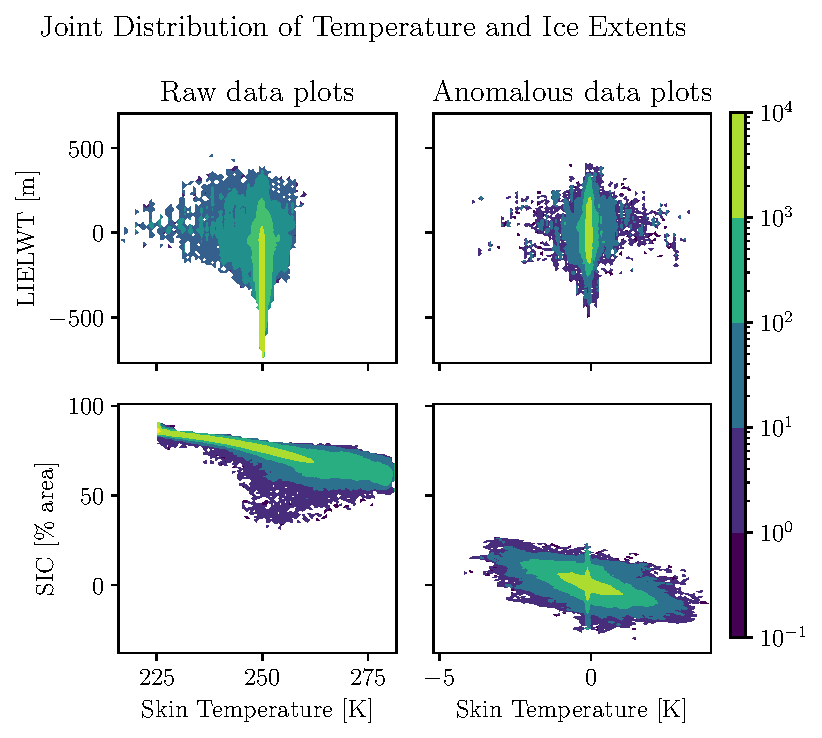
\includegraphics{images/week8/hres/distribution_of_temperature_ice_both_raw_and_anomalous.pdf}
    \caption{Distribution of skin temperature against ice. This is a 2 dimensional histogram where the colour represents the number of points in our dataset with a given temperature and amount of ice. The top row contains all the gridpoints over land, the corresponding ice values being Land Ice Liquid Water Equivalent Thickness (LILWET). And the row subplot contains all the gridpoints over the sea, with Sea ice concentration (SIC) plotted on the y-axis. The left column contains the raw values for each measurement and the right column has the anomalous values where the mean value of each variable is removed for each spatial location. (The values for this is plotted below).}
    \label{fig:joint_distribuition_temp_ice}
\end{figure}

This plot (Figure \ref{fig:joint_distribuition_temp_ice}) tells us an interesting story. For sea ice, we can observe a significant relationship between skin temperature and SIC. This relationship matches with our intuition, which is great. However land ice doesn't exhibit the same strong relationship as sea ice. This is interesting as it suggests that it is driven by a different set of processes. We will have to be careful about this in our ongoing analysis. The anomalous plots tell us a similar story in regards to the relationship between the two variables, however as the overall shape for both land and sea ice plots changed, we expect there to be some spatial variation in how we see the relationship between ice and temperature expressed.

One thing we need to remember with this plot is that it will be exhibiting some spatial bias because some locations will have higher values of ice and lower temperatures. Additionally these plots only contain data points from 2002 because the land ice data only has values from then due to it being based on an later mission. 

We can learn more about this relationship by looking at the spatial and temporal variability and trends for each of the variables.

\section[Spatial distribution of trends]{Spatial distribution of trends in Antarctic ice and temperature}

\section{Temporal variability of Antarctic ice and temperature}

\section{Regression using temperature to predict Antarctic ice}

\section{Statistics for Antarctic ice and temperature}

\section*{Things still to do for this section}
\begin{enumerate}
    \item Add to the scatter plots
    \begin{itemize}
        \item Trend lines.
        \item Statistics such as correlations
    \end{itemize}
    \item Regress temperature onto ice.
    \item Plot mean values for ice and temperature to explain removing the anomalies.
    \item Fill out red citation notes in the text.
\end{enumerate}

\end{document}